\documentclass[11pt,titlepage]{article}
\usepackage{fullpage}
\usepackage{amsmath}
\usepackage{amssymb}
\usepackage{color}
\usepackage{graphicx}
\graphicspath{ {images/} }
\usepackage{tikz}
\usetikzlibrary{shapes,arrows,positioning,calc}
\usepackage{float}
\restylefloat{table}
\usepackage{array}
\tikzset{
    block/.style = {draw, fill=white, rectangle, minimum height=3em, minimum width=3em},
    sum/.style = {draw, fill=white, circle, node distance=1cm},
    input/.style = {draw=none},
    output/.style = {draw=none},
    coord/.style = {coordinate}
}

\author{Rane Brown \\ Kate Schneider}
\title{ECEN 4638: Lab X.1PI}
\date{\today}

\begin{document}
\maketitle
\tableofcontents
\listoffigures
\newpage

\section{Description}
    This lab will further explore the Torsional Disc System using Proportional-Integral control, with the goal of designing a PI-based cruise control system that works well for inertia changes of $\pm10\%$. The controller is then tested on two different Torsional Disc apparatuses to evaluate the design for robustness. The system setup will be similar to what was used in labX.1P; only the bottom disc of the TDS will be used and the four weights will be set at a radius of 6.5cm.


\section{System Model}
   As in labX.1P, the Torsional Disc system can be modeled as an LTI system, with the below equation
    \begin{equation} \label{eq:lti}
        J\dot{\omega}+c\omega=k_hu
    \end{equation}
    Where $J=\mbox{ total system inertia}$, $\omega=\mbox{ velocity rad/sec}$, $c=\mbox{ system drag}$, $k_h=\mbox{ hardware gain}$, $u=\mbox{ reference}$.
    
    
    \subsection{Calculated Parameters}
        During labX.1P, each team calculated parameters $c$ and $k_h$ for one torsional disc system based on its experimental data. These parameters are listed in the table below.

    
            \begin{table}[h!]
            \centering
            \begin{tabular}{|m{4cm}|m{3cm}|m{3cm}|} 
                \hline
                System & $c$ &$k_h$ \\ 
                \hline
                1 &  0.0082 & 0.3577\\
                \hline
                \textbf{1} & \textbf{0.0079} & \textbf{0.3598}\\
                \hline
                2 & 0.0078 & 0.15\\
                \hline
                2 & 0.0081 & 0.376\\
                \hline
                3 & 0.0110 & 0.387\\
                \hline
                3 & 0.010 & 0.0084\\
                \hline
                4 & 0.0111 & 0.0084\\
                \hline
                4 & 0.0184 & 0.387\\
                \hline
            \end{tabular}
            \caption{Torsional Disc System Parameters} \label{table:TDS_param}
        \end{table}
        
        For a radius of 7.5 cm, the calculated total system inertia $J$ is 0.0128 $kg m^2$.
        
        For this experiment, our cruise control system was designed using the calculated parameters from Torsional Disc System 1 (in bold in the above table), and the PI controller was tested on TDS systems 1 and 4.

    \subsection{Transfer Functions}
    
	\begin{figure}[H]
	\centering
	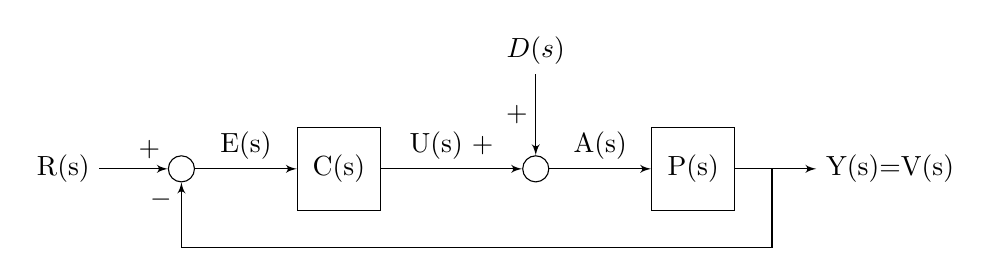
\begin{tikzpicture}[auto, node distance=2cm,>=latex']
		\node [input, name=rinput] (rinput) {R(s)};
		\node [sum, right of=rinput, node distance=1.5cm] (sum1) {};
		\node [coord, below of=sum1, node distance=1cm] (fdbk1) {};
		\node [block, right of=sum1] (controller) {C(s)};
		\node [sum, right of=controller, node distance=2.5cm] (sum2) {};
		\node [block, right of=sum2, node distance=2cm] (plant) {P(s)};
		\node [coord, right of=plant, node distance=1cm] (fdbk2) {};
		\node [coord, below of=fdbk2, node distance=1cm] (fdbk3) {};
		\node [input, above of=sum2, node distance=1.5cm] (disturbance) {$D(s)$};
		\node [output, right of=plant, node distance=2.5cm] (output) {Y(s)=V(s)};
		\draw [->] (rinput) -- node[xshift=.2cm]{$+$} (sum1);
		\draw [->] (disturbance) -- node[xshift=-.5cm]{$+$} (sum2);
		\draw [->] (sum1) --node {E(s)} (controller);
		\draw [->] (controller) -- node{U(s) $+$} (sum2);
		\draw [->] (sum2) -- node{A(s)} (plant);
		\draw [->] (plant) -- node {}(output);
		\draw [-] (fdbk2) -- (fdbk3);
		\draw [-] (fdbk3) -- (fdbk1);
		\draw [->] (fdbk1) -- node[yshift=.2cm]{$-$} (sum1);
	    \end{tikzpicture}
	\caption{Cruise Control Feedback System} \label{fig:block}
	\end{figure}
    
    	From our LTI model, we see that the system plant is modeled with the below equation.
 	\begin{equation} \label{eq:lti}
       		P(s)= \frac{k_h}{Js+c}e^{-T_ds}
    	\end{equation}
    Where $J=\mbox{ total system inertia}$, $c=\mbox{ system drag}$, $k_h=\mbox{ hardware gain}$, and $T_d=\mbox{ time delay}$.
    In this lab, we use a PI controller, $C(s)=\frac{k_I}{s}+k_p$. \\
    
    \textcolor{red}{include info from sheet on these and what they tell us!! Then add plots!!}
    There are multiple transfer functions which are of interest in our system. The first transfer function of interest is the closed-loop transfer function from reference input $R$ to output $Y$:
	\begin{equation}
		H_{yr}=\frac{Y}{R}=\frac{CP}{1+CP}=\frac{kk_I+kk_ps}{Js^2+(c+kk_p)s+kk_I}
	\end{equation}
	
	From the equation for $H_{yr}$, we can see that the DC gain of this transfer function is 1, as we would expect \textcolor{red}{because...}.
	
	Another transfer function of interest is the closed-loop transfer function from reference input $R(s)$ to controller output $U(s)$.
	\begin{align}
		H_{ur}&=\frac{U}{R}=\frac{C}{1+CP}=\frac{Jck_Ik_ps^3+Jk_Is^2+ck_Is}{Js^2+(c+kk_p)s+kk_I}
	\end{align}
	
	This transfer function has a DC gain of  $H_{ur}(0)=\frac{c}{k}$. This value represents the input that is needed to compensate parameter $c$ in steady state. 
		
	We can also look at the transfer function from the disturbance $D(s)$ to the output $Y(s)$, since again, rejecting disturbance input such as hills and bumps is important in a cruise control system.
	\begin{equation}
		H_{yd}=\frac{Y}{D}=\frac{\frac{k}{J}s}{s^2+(\frac{c}{J}+\frac{k_pk}{J}s)+\frac{k}{J}k_I}
	\end{equation}
	
	The final closed-loop transfer function of interest is $H_{ud}$, the transfer function from the disturbance $D(s)$ to the controller output $U(s)$. 
	\begin{equation}
		H_{ud}=\frac{-\frac{k}{J}(k_ps+k_I)}{s^2+(\frac{c}{J}-\frac{kk_p}{J})s+\frac{kk_I}{J}}
	\end{equation}	
		
	We will also examine the open-loop transfer function $L(s)=P(s)C(s)$, which will be useful in determining gain and phase margins of our system to ensure stability.
	
	\begin{equation}
		L(s)=P(s)C(s)=	\frac{k}{Js+c}(\frac{k_I}{s}+k_p)
		\end{equation}


\section{Matlab Analysis}\label{sec:mat_anys}
    \subsection{Time Domain}
	    Before implementing our PI controller on a physical TDS, we can formulate and test the design in Matlab to ensure the system meets certain time and frequency domain specifications. In the time domain, relevant specifications include rise time $t_r$, settling time $t_s$, and overshoot $M_p$. Choosing desired ranges for these parameters allows us to estimate $\zeta$ and $\omega_{n}$ for a simple second-order system of the form
	    
	    \begin{equation}
	    	\frac{K\omega_n^2}{s^2+2\zeta \omega_ns+\omega_{n}^2}
	    \end{equation}
	    
	    with the relationships 
	    \begin{equation}
	    	t_r = \frac{1.8}{\omega_n}, \hspace{1cm} t_s=\frac{4.6}{\zeta\omega_n},  \hspace{1cm}  M_p=e^{\frac{-\pi \zeta}{\sqrt{1-\zeta^2}}}
	    \end{equation}
    
    	However, when using these estimates, we must keep in mind that our PI controller also introduces an additional zero to the closed-loop transfer function $H_{yr}(s)$ which will affect the time domain response of our system. Most notably this zero will increase $M_p$ and decreasing $t_r$. Thus, design must aim for a larger $\zeta$, while $\omega_n$ can be decreased slightly and still meet rise time specifications. \\
    
    	If, for instance, we choose desired values of $t_r<1 sec$, $t_s < 5 sec$, and $M_p<10\%$, we can estimate suitable $\omega_n$ and $\zeta$ for $H_{yr}(s)$ by hand calculation, then model the system in Matlab. Iterating on the design in Matlab allows us to fine-tune the controller, which we can then evaluate on the physical system.\\
	\textcolor{red}{discuss/plot all the other transfer functions!!!}
	
	The specifications above results in the values $\omega_n = , \hspace{1cm} \zeta= $ which gives values $k_I= , k_p= $. This results in the system transfer function $H_{yr}(s) = $. The step response plot for $H_{yr}(s)$ is given below.
	
	\textcolor{red}{add plot here}
	
	The additional zero results in a greater overshoot and overall faster response. The plots of the other three transfer functions of interest are included below. \textcolor{red}{add other TF plots here}
	
	We can further refine our design in order to get a better time domain response from our system, now that we have observed the effect of the additional zero in Matlab simulations. \textcolor{red}{include one more iteration, with better params which worked for the exp sys.}
	
    \subsection{Frequency Domain}
    	In addition to time domain specifications, certain aspects of a system's frequency domain response are important to take into consideration to ensure the stability and good performance of that system. These values are the steady-state error, $e_{ss}$, the phase margin $PM$, the gain margin $GM$, and the bandwidth,, which gives us the system's half-power frequency. $e_{ss}$ and  $\omega_{BW}$ are important for system performance. $PM$, and $GM$ ensure stability of the system, with $45<PM<60$ an ideal region for the phase margin, $GM>$ a good goal for gain margin. 
	
	We can plot the frequency response of our first system () and analyze the stability and performance of the system. Note that we have 
	$PM=$, $GM=$, $\omega_{BW}=$, and $e_{ss}=$. \textcolor{red}{discuss what these mean, then do an iteration using freq plots. FINALLY, put all of these together into a system that has good time and freq response characteristics in Matlab. Make sure for this system you plot several other transfer functions as well - use one that may have performed well on the TDS itself - then add in $+-10-\%$ on the J value and discuss how that worked out.}
	 
\section{Experimental Analysis}
    After conducting the matlab analysis in section \ref{sec:mat_anys} experimental data was collected from two different torsion disc systems. Data was collected from two systems in order to examine the robustness of the PI controller and make any necessary adjustments.
    \subsection{Setup}
    The first step in collecting experimental data was to select a rise time ($t_r$) and overshoot ($M_p$) for the system. As an initial starting point values of $t_r = 0.5$ sec and $M_p = 5\%$ were selected. Using these values the damping $\zeta$ and natural frequency $\omega_n$ were calculated using equations \ref{eq:zeta} and \ref{eq:omega}
    \begin{align}
        \zeta &= \frac{|\ln(0.05)|}{\sqrt{\pi^2+[ln(0.05)]^2}} = 0.69 \label{eq:zeta} \\[1em]
        \omega_n &= \frac{1.8}{0.5} = 3.6 \label{eq:omega}
    \end{align}
    These values were used as an initial starting point and adjustments were made based on the response calculated in matlab and the corresponding response on the TDS. In cases where the overshoot became too high the damping was increased. It also became necessary to increase the bandwidth of the system in order to reduce the noise on the live system. Table \ref{table:respData} shows the various calculated values based on necessary changes. For each iteration the value in bold was adjusted to improve the response. The adjustments were determined based on the response of the system to a step input as outlined in section \ref{sub:step} and to a ramp disturbance in section \ref{sub:dist}.
    \begin{table}[H]
        \centering
        \begin{tabular}{|m{1.5cm}|m{1.5cm}|m{1.5cm}|m{1.5cm}|m{1.5cm}|m{1.5cm}|m{1.5cm}|m{1.5cm}|} 
            \hline
            Test & $M_p$ & $t_r$ & $\zeta$ & $\omega_n$ & $K_p$ & $K_I$ & $BW$ \\ 
            \hline
            test1 & \textbf{5.00} & \textbf{0.50} & 0.69 & 3.60 & 0.1548 & 0.4611 & 6.55 \\
            \hline
            test2 & 19.58 & 0.090 & 0.69 & \textbf{10} & 0.469 & 3.558 & 19.55 \\
            \hline
            test3 & 16.23 & 0.085 & \textbf{0.80} & 10 & 0.5472 & 3.558 & 20.948 \\
            \hline
            test4 & 14.67 & 0.039 & \textbf{0.90} & \textbf{20} & 1.258 & 14.23 & 45.59 \\
            \hline
            test5 & 13.63 & 0.038 & \textbf{0.95} & 20 & 1.329 & 14.23 & 47.00 \\
            \hline
            test6 & 13.92 & 0.025 & 0.95 & \textbf{30} & 2.006 & 32.018 & 71.08 \\
            \hline
        \end{tabular}
        \caption{System Response} \label{table:respData}
    \end{table}

    \subsection{Time Domain - Step Response} \label{sub:step}
    The values shown in table \ref{table:respData} were calculated from the closed loop transfer function of the system model. The ideal step response from matlab was then compared to experimental data from the TDS. This experimental data was collected by adjusting the $K_p$ and $K_I$ values in Labview and saving the response data to a text file. Data was collected for TDS machine 1 and TDS machine 4.
    \begin{figure}[H]
        \centering
        \begin{minipage}{.5\textwidth}
            \centering
            \includegraphics[scale=.3]{stepM1_T1}
            \caption{Step Response m1t1}
            \label{fig:stepM1_T1}
        \end{minipage}%
        \begin{minipage}{.5\textwidth}
            \centering
            \includegraphics[scale=.3]{stepM1_T2}
            \caption{Step Response m1t2}
            \label{fig:stepM1_T2}
        \end{minipage}%
    \end{figure}
    \begin{figure}[H]
        \centering
        \begin{minipage}{.5\textwidth}
            \centering
            \includegraphics[scale=.3]{stepM1_T3}
            \caption{Step Response m1t3}
            \label{fig:stepM1_T3}
        \end{minipage}%
        \begin{minipage}{.5\textwidth}
            \centering
            \includegraphics[scale=.3]{stepM1_T4}
            \caption{Step Response m1t4}
            \label{fig:stepM1_T4}
        \end{minipage}%
    \end{figure}
    \begin{figure}[H]
        \centering
        \begin{minipage}{.5\textwidth}
            \centering
            \includegraphics[scale=.3]{stepM1_T5}
            \caption{Step Response m1t5}
            \label{fig:stepM1_T5}
        \end{minipage}%
        \begin{minipage}{.5\textwidth}
            \centering
            \includegraphics[scale=.3]{stepM1_T6}
            \caption{Step Response m1t6}
            \label{fig:stepM1_T6}
        \end{minipage}%
    \end{figure}
    \begin{figure}[H]
        \centering
        \begin{minipage}{.5\textwidth}
            \centering
            \includegraphics[scale=.3]{stepM4_T1}
            \caption{Step Response m4t1}
            \label{fig:stepM4_T1}
        \end{minipage}%
        \begin{minipage}{.5\textwidth}
            \centering
            \includegraphics[scale=.3]{stepM4_T2}
            \caption{Step Response m4t2}
            \label{fig:stepM4_T2}
        \end{minipage}%
    \end{figure}
    \begin{figure}[H]
        \centering
        \begin{minipage}{.5\textwidth}
            \centering
            \includegraphics[scale=.3]{stepM4_T3}
            \caption{Step Response m4t3}
            \label{fig:stepM4_T3}
        \end{minipage}%
        \begin{minipage}{.5\textwidth}
            \centering
            \includegraphics[scale=.3]{stepM4_T4}
            \caption{Step Response m4t4}
            \label{fig:stepM4_T4}
        \end{minipage}%
    \end{figure}
    \begin{figure}[H]
        \centering
        \includegraphics[scale=.3]{stepM4_T5}
        \caption{Step Response m4t5}
        \label{fig:stepM4_T5}
    \end{figure}
    \noindent Figures \ref{fig:stepM1_T1} through \ref{fig:stepM1_T6} show the plots of the matlab data and the collected experimental data for machine 1. Figures \ref{fig:stepM4_T1} to \ref{fig:stepM4_T5} show the data comparisons for machine 4. From this information it is possible to calculate the actual rise time and overshoot of the system for different $K_I$ and $K_p$ values. Table \ref{table:stepComp} shows the calculated $t_r$ and $M_p$ values.
    \begin{table}[H]
        \centering
        \begin{tabular}{|m{2cm}|m{2cm}|m{2cm}|m{2cm}|m{2cm}|m{2cm}|} 
            \hline
            matlab $t_r$ & mach1 $t_r$ & mach4 $t_r$ & matlab $M_p$ & mach1 $M_p$ & mach4 $M_p$\\ 
            \hline
            0.275 & 0.09 & 0.19 & 16.646 & 29.78 & 54.66 \\ 
            \hline
            0.09 & 0.05 & 0.05 & 19.58 & 54.58 & 46.45 \\ 
            \hline
            0.085 & 0.05 & 0.03 & 16.23 & 51.71 & 73.95 \\ 
            \hline
            0.039 & 0.03 & 0.03 & 14.67 & 71.97 & 71.37 \\ 
            \hline
            0.038 & 0.03 & 0.03 & 13.63 & 70.93 & 77.01 \\ 
            \hline
            0.025 & 0.02 & n/a & 3.916 & 101.66 & n/a \\ 
            \hline
        \end{tabular}
        \caption{$t_r$ and $M_p$ Comparison} \label{table:stepComp}
    \end{table}
    \noindent The overshoot amounts for the proportional integral controller quickly become large. Even with maximum damping it was not possible to reduce the overshoot by the desired amount. This large overshoot was partly due to increasing the natural frequency to reduce the steady state noise. With more iterations and experiments it would be possible to get a slightly better response.

    \subsection{Time Domain - Disturbance} \label{sub:dist}
    Another important aspect of of designing the PI controller was viewing the response of the system to a ramp disturbance. As shown from the transfer functions and calculations in section \ref{sec:tf} there should be a constant steady state error to a ramp disturbance. As seen in figures \ref{fig:distm1} and \ref{fig:distm4} there is a constant error to a ramp disturbance on the physical system as expected. In the plots the response with no disturbance is shown in blue and the response to the ramp disturbance is shown in orange.
    \begin{figure}[H]
        \centering
        \includegraphics[scale=.5]{m1dist}
        \caption{Ramp Distrubance m1}
        \label{fig:distm1}
    \end{figure} 
    \begin{figure}[H]
        \centering
        \includegraphics[scale=.5]{m4dist}
        \caption{Ramp Distrubance m4}
        \label{fig:distm4}
    \end{figure} 

\section{PI Controller Design Summary}
    Designing a PI controller is a complex and iterative process as outlined in the above sections. Analyzing a model of they system using matlab is a starting point that can provide some useful information. For example, viewing the various transfer functions helps to provide a baseline for the expected response to different inputs and disturbances. Calculated system parameters such as overshoot, rise time, natural frequency, and damping provide initial $K_p$ and $K_I$ values. On the actual TDS the response varies from the simulation due to variables that are not present in the ideal model. Iteratively updating system values gradually improves the system response but a PI controller is not sufficient to eliminate all undesirable characteristics. Further labs will explore more complex controllers which will continue to improve the response characteristics.


\end{document}